\documentclass[../../main.tex]{subfiles}

\begin{document}
In order to analyse and the pan-tilt system and design appropriate controllers, a mathematical model describing the dynamics of a DC motor has to be derived. First the electric equivalent circuit of the DC motor is analysed. As seen in figure \ref{fig:Armature_Circuit} the motor can be described as a voltage source in series with a resistor, $R_m$, an inductor, $L_m$, and another voltage source representing the \textit{back emf}. To setup the system equation it is assumed that the torque is proportional to the angular velocity of the motor shaft. Furthermore, it is assumed that the motor torque is proportional to the current, $i$. If the motor torque and the back emf constant are represented in SI units, they are equal to each other \cite{universityofmichigan2019}. This constant will henceforward be denoted as one constant, $K_m$. The system equations is derived using figure \ref{fig:Armature_Circuit} as well as Newtons's second law and Kirchoff's voltage law. The equations can be seen in equation \ref{eq:sysEq1} and \ref{eq:sysEq2}.

\begin{equation}
    J\ddot{\theta}+b\theta = K_m i
    \label{eq:sysEq1}
\end{equation}

\begin{equation}
    L_m \frac{di}{dt} + R_m i = V -K_m \dot{\theta}
    \label{eq:sysEq2}
\end{equation}

\begin{table}[]
    \centering
    \begin{tabular}{L{6 cm} L{0.5 cm}  C{1.5 cm} | C{3 cm} C{3 cm}}
        \textbf{Parameter} &  & \textbf{Unit} &  \textbf{Pan} &  \textbf{Tilt} \\ \hline
        Moment of inertia & $J$ & [\si{\kilogram\square\meter}] & 0.02 & \num{5.6e-3}\\
        Inductance & $L_m$ & [\si{\henry}] & \num{2.75e-6} & \num{2.75e-6}\\
        Resistance & $R_m$ & [\si{\ohm}] & 4.65 & 4.65 \\
        Back emf/motor torque constant
        & $K_m$ & [??] & 0.49 & 0.49 \\
        Viscous friction constant & $b$ & [\si{\newton\meter\second}] & \num{7.38e-4} & \num{7.38e-4}  \\
        
    \end{tabular}
    \caption{Parameters used for modelling the pan and tilt motor. $R_m$, $K_m$, and $b$ is found experimentally, $J$ is estimated and $L$ is from \cite{universityofmichigan2019}.}
    \label{tab:modellingParam}
\end{table}

Using equation \ref{eq:sysEq1} and \ref{eq:sysEq2} the system is represented on state space form seen in equation \ref{eq:stateSpaceSys1}.
\begin{equation}\label{eq:stateSpaceSys1}
\begin{split}
\begin{bmatrix}
\dot{\theta}\\
\ddot{\theta}\\
\dot{i}
\end{bmatrix} &=
\begin{bmatrix}
0 & 1 & 0 \\
0 & \frac{-b}{J} & \frac{K_m}{J}\\
0 & \frac{-K_m}{L} & \frac{-R_m}{L_m}
\end{bmatrix}
\begin{bmatrix}
\theta\\
\dot{\theta}\\
i
\end{bmatrix}
+ 
\begin{bmatrix}
0 \\
0 \\
\frac{1}{L}
\end{bmatrix} \\
    y &= 
    \begin{bmatrix}
    1 & 0 & 0\\
    0 & 1 & 0
    \end{bmatrix}
    \begin{bmatrix}
    \theta\\
    \dot{\theta}\\
    i
    \end{bmatrix}
    \end{split}
\end{equation}

The system dynamics can also be described by the transfer functions for velocity and position, seen in equation \ref{eq:tf_pos_vel} and \ref{eq:tf_pos}.
\begin{equation}\label{eq:tf_pos}
    \frac{\dot{\theta}(s)}{V(s)} = \frac{K_m}{(J\cdot s + b)(L\cdot s + R) + K_m^2}
\end{equation}

\begin{equation}
    \frac{\theta(s)}{V(s)} = \frac{K_m}{s\cdot((J\cdot s + b)(L\cdot s + R) + K_m^2)} \qquad 
\end{equation}


\begin{figure}[H]
    \centering
    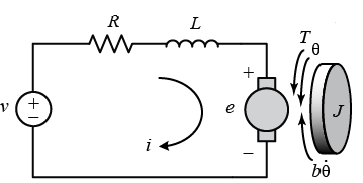
\includegraphics[width=0.6\textwidth]{Sections/System_Modelling/Images/Armature_Layout.PNG}
    \caption{Electrical equivalent circuit diagram of a DC motor and a free-body diagram of the motor shaft. T represents the motor torque, J the inertia of the motor, $\theta$ the position of the shaft and $b\dot{\theta}$ the friction torque. \cite{universityofmichigan2019}}
    \label{fig:Armature_Circuit}
\end{figure}







\subsection{Determining System Parameters}\label{subsec:motorParameters}
\subsubsection*{Moment of Inertia}
Moment of inertia, sometimes referred to as mass moment of inertia, is the angular motion analogue to mass in a translational system. It determines proportionality between the applied torque and the angular acceleration. An estimation for the value of the moment of inertia will be calculated based on measurements and information from data sheets. 

To estimate the inertia, a simplified representation of the pan and tilt system, in figure \ref{}, is considered. This representation ignores bolts, brackets, gears, etc. Furthermore, the extrusions are considered as solid boxes, thus ignoring the profile shape.

Based on the simplified representation, the inertia accruing to the tilt frame around the axis $a_{tilt}$ can be found. Using a formula to calculate the inertia of a box with dimensions $w_t\times l_t\times h_t$ and subtracting the inertia of the inner box of dimensions $w_{ct}\times l_{ct}\times h_t$, equation \ref{eq:J_tilt} is found, where $\rho_t$ is the density of the tilt frame.

\begin{equation} \label{eq:J_tilt}
    J_{a_{tilt}} =  w_{t} \,h_{t}\, l_{t}\,\rho_{t}\frac{1}{12}(l_{t}^2+h_{t}^2)-w_{ct}\, h_{t} \, l_{ct} \, \rho_{t}\frac{1}{12}(h_{t}^2+l_{ct}^2)
\end{equation}

The inertia of the pan frame can be found in a similar manner, however to properly estimate the inertia accruing to the pan motor, the tilt frame must be considered as well. The inertia of the tilt frame about the axis $a_{pan}$ also depends on the angle, $\theta$, at which the tilt motor is positioned.

The same approach of subtracting the inertia of an inner box from an outer box can be used, but since no formula is readily available for calculating the inertia of an inclined box, integration must instead be used. The inertia of a point mass is defined as $J=m\cdot r^2$ \cite{PrincipalsOfPhysics}, where $m$ is the mass of the point and $r$ is the distance from the point to the axis of rotation. Thus the inertia of a volume, $V$, can be found as $\iiint_V \rho r^2 dV$, where $\rho$ is the density of the volume and $r$ is a function that describes the distance to the axis of rotation at each point in the volume. In the case of the box positioned as in figure \ref{}, $r$ can be described as in equation \ref{eq:r_function}.
\begin{equation}\label{eq:r_function}
    r = \sqrt{x^2\cos{\theta}^2+x^2\sin{\theta}^2+(y\cos{\theta}-z\sin{\theta})^2}
\end{equation}
Integrating over the dimensions of the inclined box, $J_{inc}$, the inertia can be found in equation \ref{eq:inc_box_inertia}.
\begin{equation}\label{eq:inc_box_inertia}
    J_{inc} = \int_{-\frac{w}{2}}^{\frac{w}{2}}
        \int_{-\frac{h}{2}}^{\frac{h}{2}}
        \int_{-\frac{l}{2}}^{\frac{l}{2}}
        \rho \cdot r^2 \,dz \,dx \,dy = \frac{1}{24}h\,l\,w\, \rho (h^2+l^2+2w^2+(h^2-l^2)\cos{2\theta})
\end{equation}
Since this function is non-linear, it will not be useful when analysing the system and designing controllers. The resulting effect of the position of the tilt frame is at a maximum, when the angle is $\theta_{t}=\frac{\pi}{2}$ and a minimum at $\theta_t=0$. Therefore it is chosen to evaluate the system at the point $\theta_t = \frac{\pi}{4}$, to get a value which is right in the middle of the two extremes. The result is shown in equation \ref{eq:inertia_lin}.

\begin{equation}\label{eq:inertia_lin}
    J_{inc,\,lin} = \frac{1}{24}h\,l\,w\, \rho (h^2+l^2+2w^2)
\end{equation}

The total inertia, $J_{a_{pan}}$, can then be found in equation \ref{eq:pan_axis_inertia}, where $J_{p\,a_{pan}}$ is the inertia of the pan frame and $J_{t\,a_{pan}}$ is the inertia of the tilt frame, both about the pan axis $a_{pan}$.

\begin{equation}\label{eq:pan_axis_inertia}
\begin{split}
        J_{p,\,a_{pan}} &= w_{p}\,l_{p}\,h_{p}\,\rho_{p}\frac{1}{12}(h_{p}^2+w_{p}^2)-w_{cp}\,l_{cp}\,h_{p}\,\rho_{p}\frac{1}{12}(h_{p}^2+w_{cp}^2) \\
        J_{t,\,a_{pan}} &= \frac{1}{24}h_t\,l_t\,w_t\, \rho_t (h_t^2+l_t^2+2w_t^2)-\frac{1}{24}h_t\,l_{ct}\,w_{ct}\, \rho_t (h_t^2+l_{ct}^2+2w_{ct}^2)
        \\
        J_{a_{pan}} &= J_{p\,a_{pan}} + J_{t\,a_{pan}}
\end{split}
\end{equation}
The densities $\rho_t = \SI{987.7 }{\kilo \gram \per \cubic \meter }$ and $\rho_p = \SI{996.3 }{\kilo \gram \per \cubic \meter } $ are based on values found from technical data of similar aluminium extrusions \cite{extrusion45x45} \cite{extrusion40x40}.
Evaluating using these values, and the measurements in figure \ref{} it is found that $J_{a_{pan}} = \SI{0.0602}{\kilo \gram \square \meter } $ and $J_{a_{tilt}} = \SI{0.0169}{\kilo \gram \square \meter }$. Since the model is based on the angular motion for the motor shaft, and not the angular motion of the pan and tilt frames, these values will have to be divided by three. This is because of the gear ratios which dictate that the pan and tilt frames have one third the angular velocity of the motor shaft for the respective frames.






\subsubsection*{ Motor Coefficients }
The coefficients of the tilt motor are found experimentally, with the approach described in the Danish article "Modeldannelse" \cite{PalleAndersenModeldannelse}. Same parameters are assumed for the pan motor. In this approach, the angular velocity and current is measured for different voltages. Equation \ref{eq:motor_coefficients} can be used to describe the relationship between the angular velocity, current and voltage, the armature voltage, $u_a$, and the external load, $\tau_b$ for the motor:
\begin{equation}\label{eq:motor_coefficients}
    \begin{split}
    \omega_{1} K + i_{a1} R_{a} &= u_{a1}  \\
    i_{a1} K - \tau_{c} - \omega_{1} b &= \tau_{b1} \\
    \omega_{2} K + i_{a2} R_{a} &= u_{a2} \\
    i_{a2} K - \tau_{c} - \omega_{2} b &= \tau_{b2} \qquad ,
    \end{split}
\end{equation}
where $K$ is a coefficient related to the torque of the motor, $\tau_{c}$ is the static friction, $b$ is the dynamic friction in the system and $R_{a}$ is the internal resistance in the motor windings. $\tau_{b1} = \tau_{b2} = 0$ when the motor is not operating with a load and the voltage is varied. $\omega_{1}$ and $i_{a1}$ are the angular velocity and current respectively at the voltage $u_{a1}$, while $\omega_{2}$ and $i_{a2}$ are a different set of angular velocity and current measurements at the voltage $u_{a2}$. For the experiment 7 different sets of angular velocity, voltage and current measurements are taken and a linear expression is fitted to the results. From the linear expression two sets of values for voltage, current and angular velocity is extracted for the computation of the motor coefficients. Further results and calculations can be seen in the digital appendix outlined in section \ref{sec:digital_appendix}. The parameter values found can be seen in table \ref{tab:modellingParam}. $\tau_c = \SI{0.139}{\newton}$ is not included as the static friction is ignored for the dynamic model.





\subsection{Analysis of the Modelled Plant}
Through discussion with the project supervisor, it has been decided that determining the inductance $L_m$ is not of interest. Instead the value found in the control tutorial \cite{universityofmichigan2019}, provided by the supervisor, is used.

The state space model in equation \ref{eq:stateSpaceSys1} combined with the model parameters from table \ref{tab:modellingParam} is used to calculate the step response and pole locations for the plant seen in figures \ref{fig:polesPlant} and \ref{fig:StepVelPlant}.

Analysing the location of the poles, it is apparent that each plant consist of one fast pole and two slower poles. This also complies well with the fact that the plant is comprised of an electrical part and a mechanical part. The electrical part is by nature significantly faster than the mechanical part, therefore yielding the fastest pole. For the dynamics of the system these fast poles are negligible, as the slower poles are dominant. Looking at the zoomed in plot in figure \ref{fig:polesPlant} it can also be seen that the difference in inertia between the two plants manipulates the second fastest pole. Since the tilt frame has a lower moment of inertia, it can be seen that the system becomes faster as the moment of inertia decreases.

% \begin{figure}
%     \centering
%     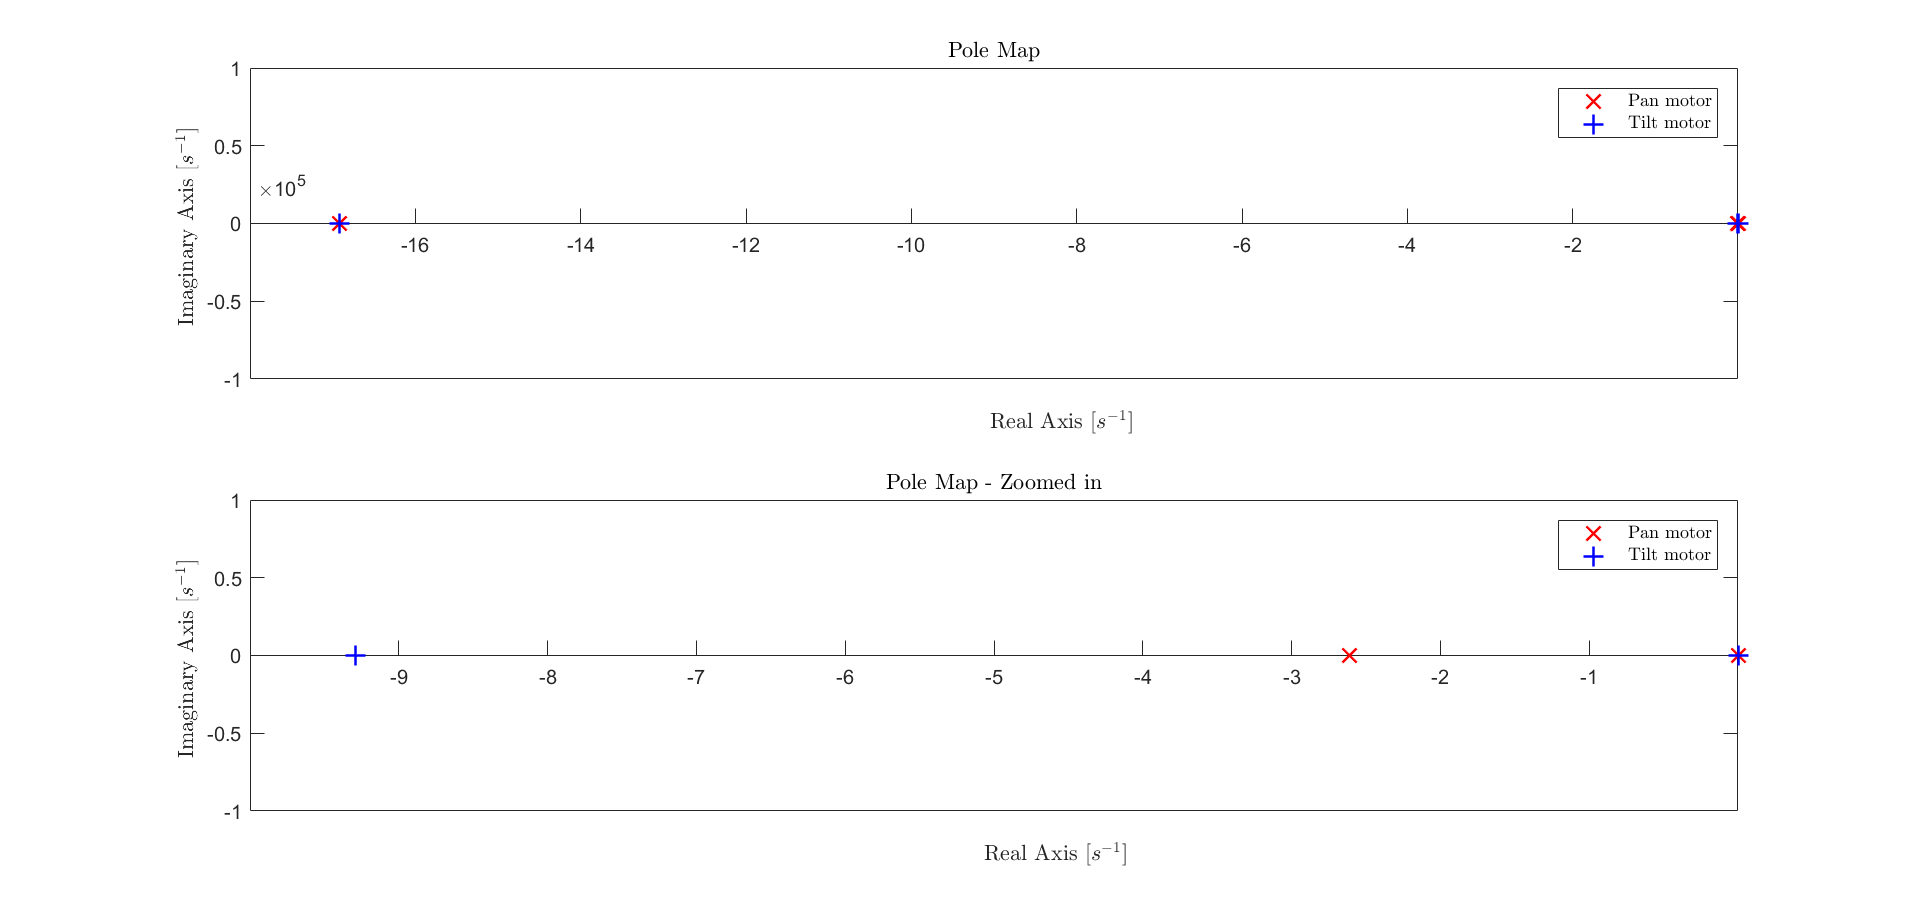
\includegraphics[width = 0.9\textwidth]{Sections/System_Modelling/Images/polesPlant.png}
%     \caption{Placement of poles for the plant.}
%     \label{fig:polesPlant}
% \end{figure}

\begin{figure}
\centering
\begin{minipage}{.5\textwidth}
  \centering
  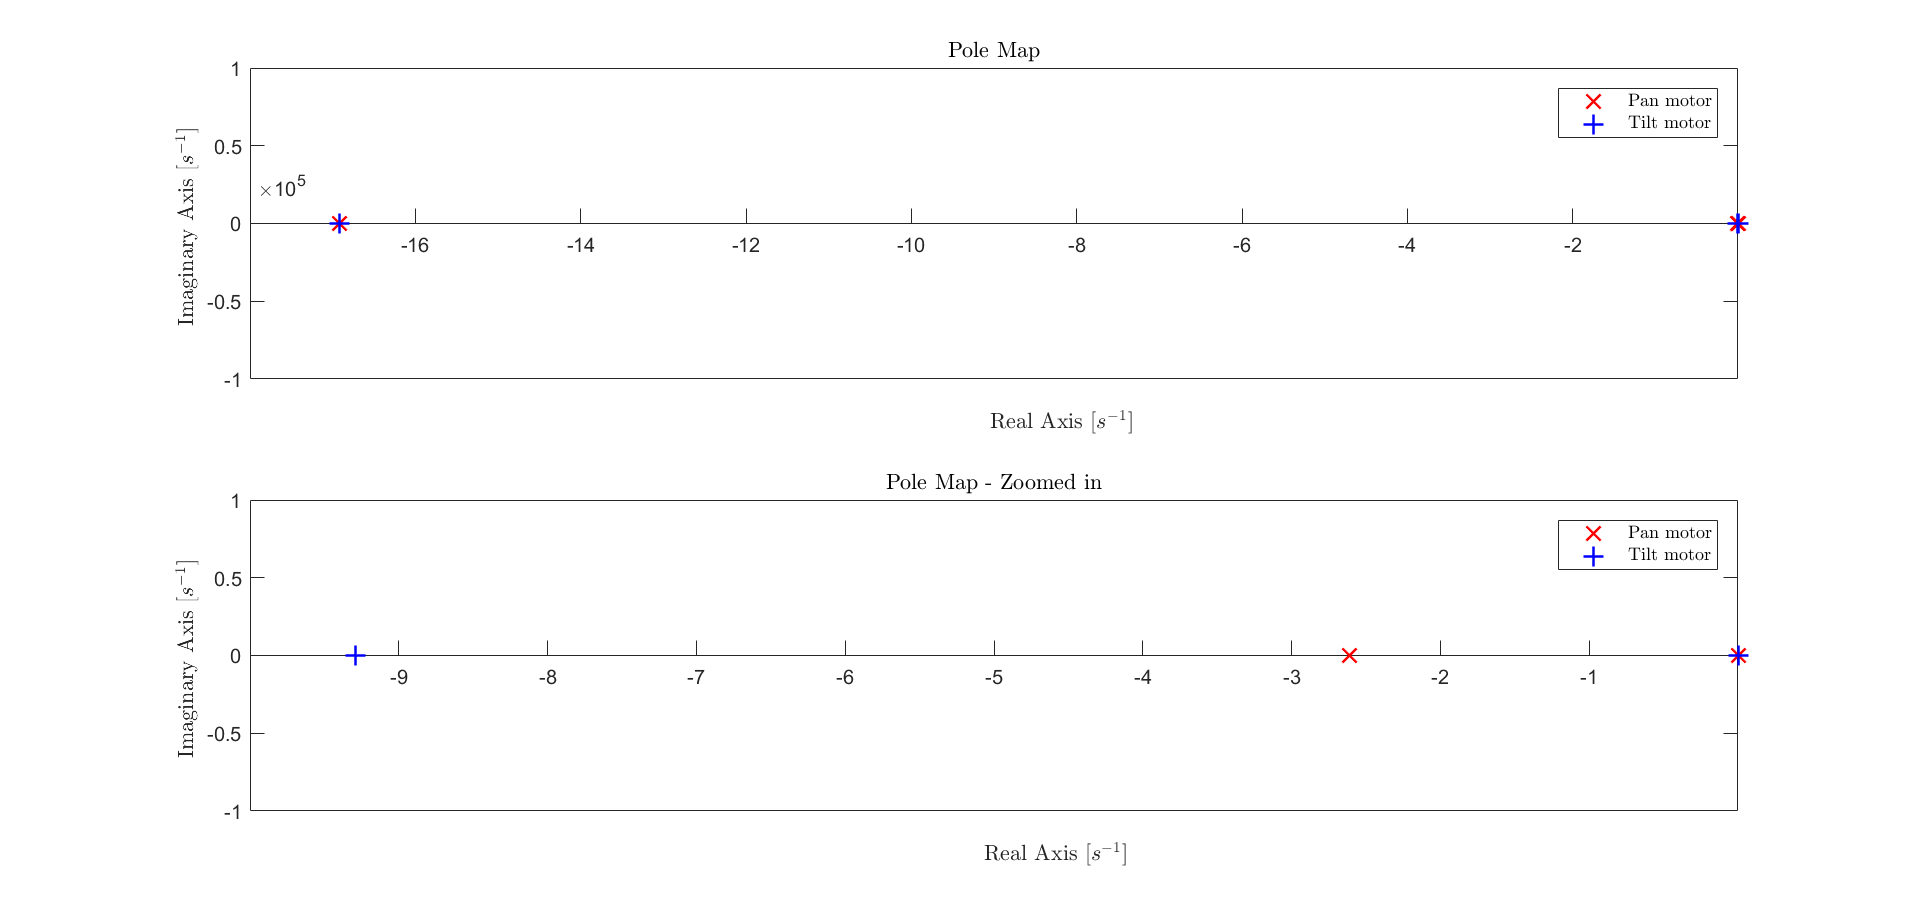
\includegraphics[width = 0.99\textwidth]{Sections/System_Modelling/Images/polesPlant.png}
  \captionof{figure}{Placement of poles for the plant.}
      \label{fig:polesPlant}
\end{minipage}%
\begin{minipage}{.5\textwidth}
  \centering
  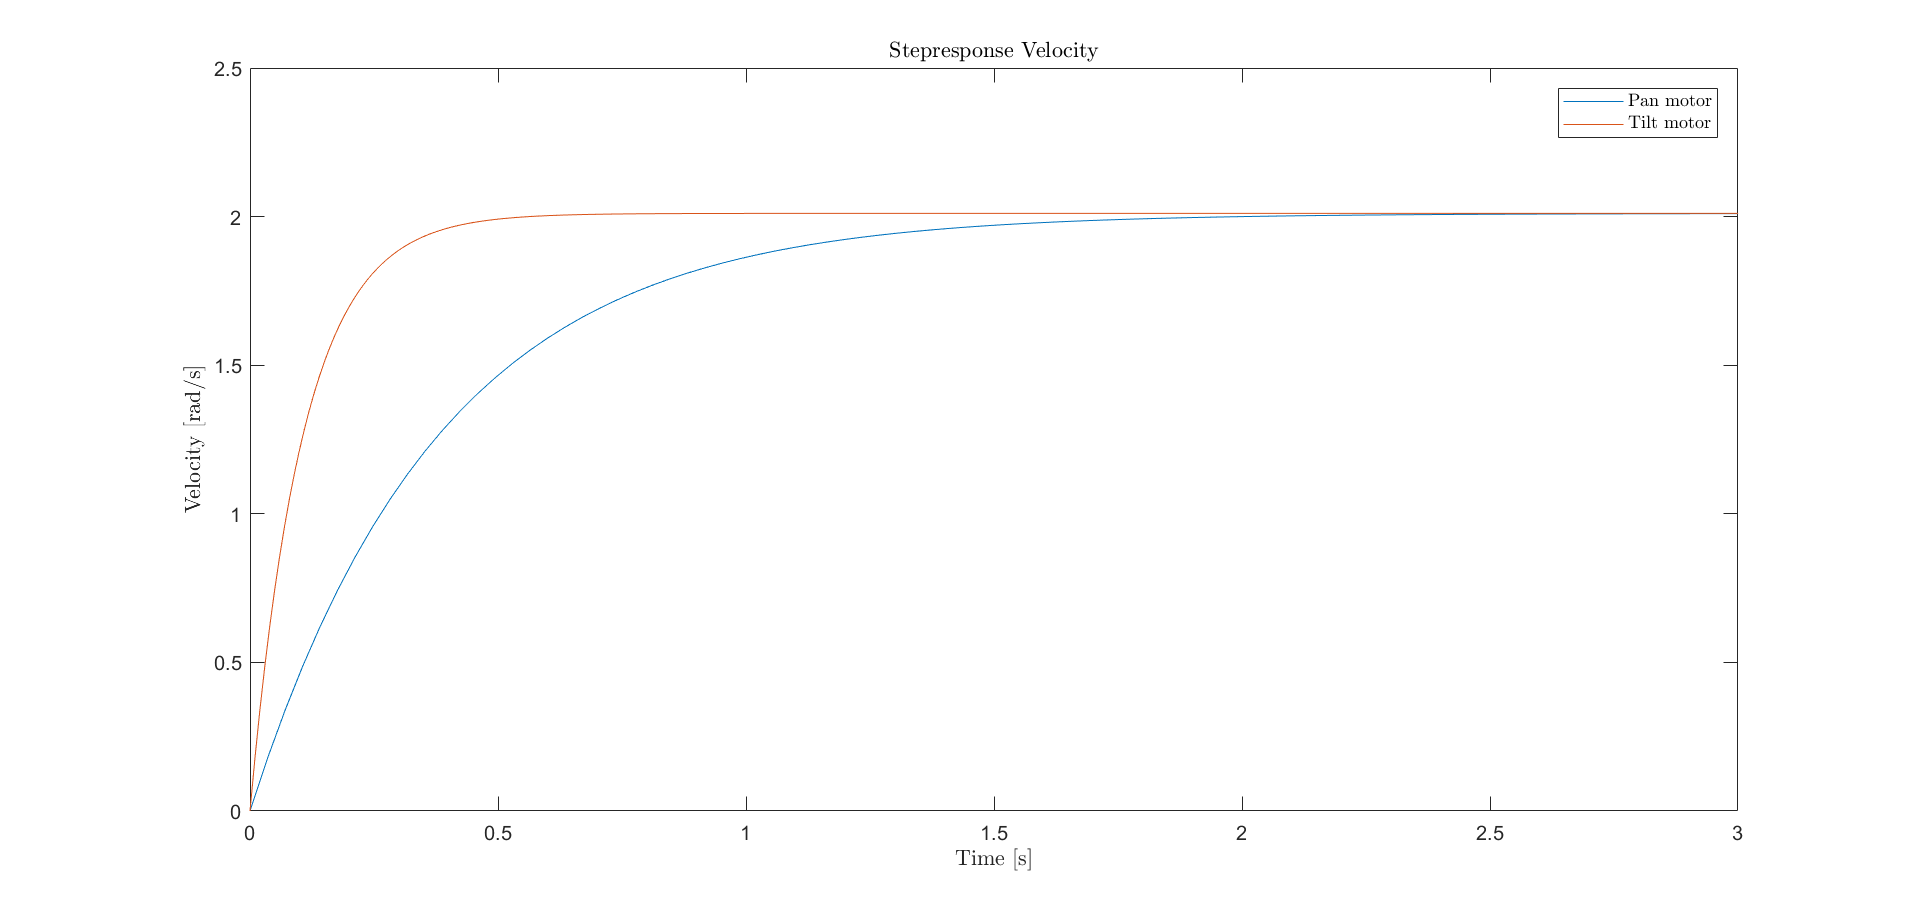
\includegraphics[width = 0.99 \textwidth]{Sections/System_Modelling/Images/stepResponseVelPlant.png}
  \captionof{figure}{Velocity step response for the plant.}
  \label{fig:StepVelPlant}
\end{minipage}
\end{figure}


The observations based on the pole locations can be verified by looking at the step response for the velocity of the systems. From figure \ref{fig:StepVelPlant} it is seen that the velocity responses resemble that of a first order system, although the transfer function for the velocity would be of second order. Thus it is verified that the fast pole for each plant is negligible. It can also be seen that the response of the tilt motor is significantly faster.
%Analysing the step response for both the plants it resembles that both plants are of first order. Though on figure \ref{fig:polesPlant} it is seen that both plants has three poles and is therefore of second order. This behavior is due to the pole introduced by the electrical system being placed so far from the other poles, that this pole becomes insignificant. Looking at figure \ref{fig:StepVelPlant}, it is seen that the pan plant is slower than the tilt due to the increased moment of inertia.  
 

% \begin{figure}
%     \centering
%     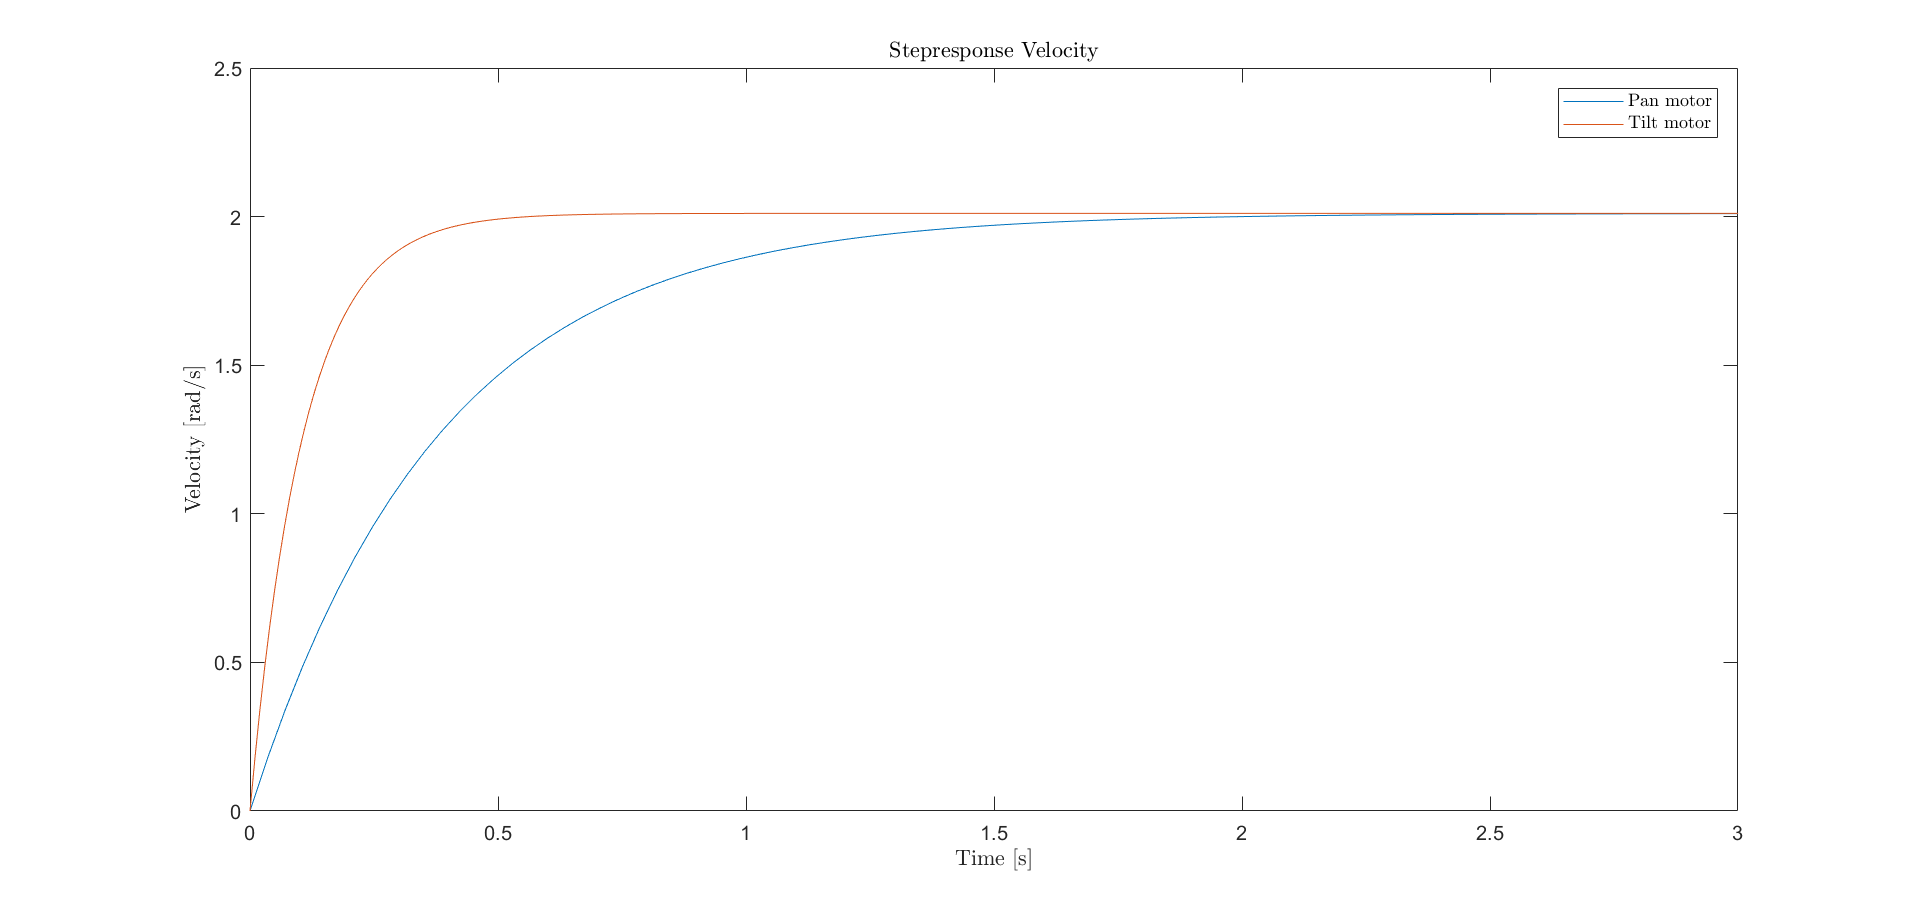
\includegraphics[width = 0.9 \textwidth]{Sections/System_Modelling/Images/stepResponseVelPlant.png}
%     \caption{Velocity step response for the plant.}
%     \label{fig:StepVelPlant}
% \end{figure}



\subsection{Conclusion}

A mathematical model of the dynamics of the DC-motors in the pan-tilt system has been derived. The moment of inertia has been estimated from equations, which describe the moment of inertia for shapes similar to the ones found in the pan-tilt system. The coefficients describing the behaviour of the DC-motor has been determined experimentally by evaluating related measurements of current, voltage and angular velocity. From the mathematical model the system is put on state space form in order to calculate step responses and analyse the location of the poles.



\end{document}